\begin{flushright} {\tiny {\color{gray} mms\_jolm17.tex}} \end{flushright}
%~~~~~~~~~~~~~~~~~~~~~~~~~~~~~~~~~~~~~~~~~~~~~~~~~~~~~~~~~~~~~~~~~~~~~~~~~~~~~~~~~~~~~~~~~~~~~~~~~~

This benchmark comes from John \etal \cite{jolm17}.
The domain is once again the unit square. The velocity field has the form of a large vortex.
Note that velocity field is actually the same velocity field as in the Donea \& Huerta benchmark above 
(albeit multiplied by a factor 100).

\begin{eqnarray}
u(x,y) &=& 200x^2(1-x)^2y(1-y)(1-2y) \\
v(x,y) &=& -200x(1-x)(1-2x)y^2(1-y)^2 \\
p(x,y) &=& 10\left[(x-1/2)^3y^2+(1-x)^3(y-1/2)^3 \right]
\end{eqnarray}

\begin{center}
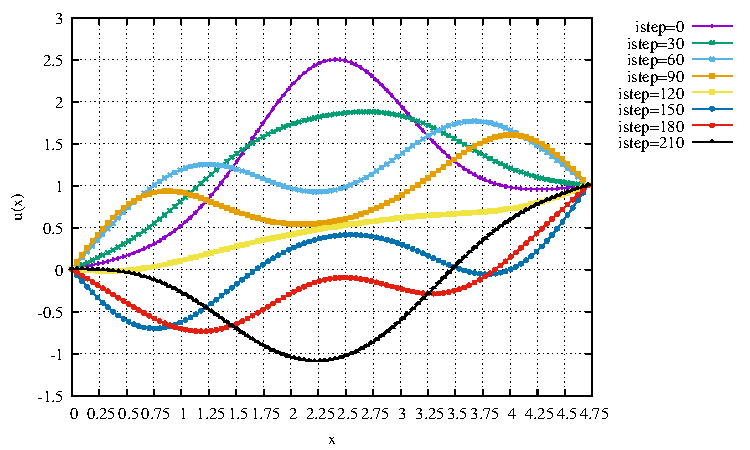
\includegraphics[width=4.5cm]{images/benchmark_jolm17/u.pdf}
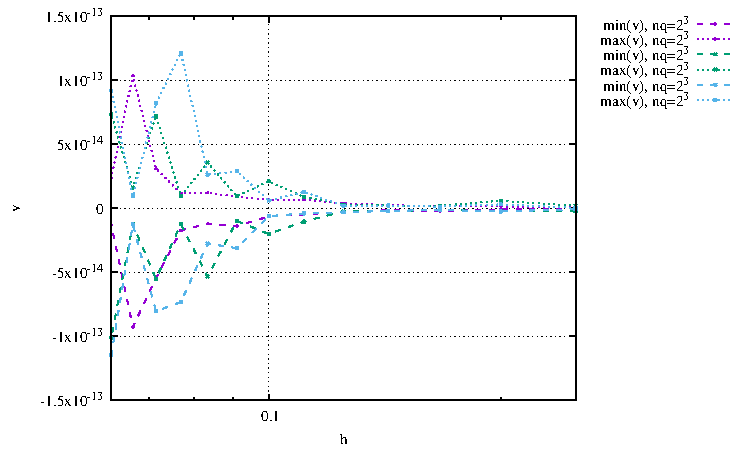
\includegraphics[width=4.5cm]{images/benchmark_jolm17/v.pdf}
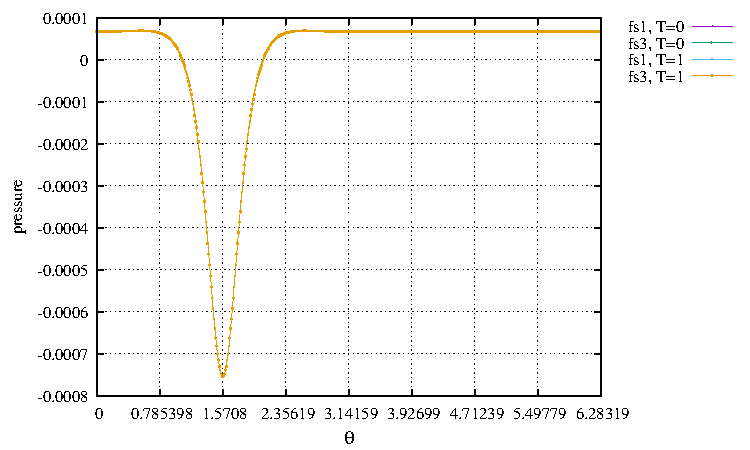
\includegraphics[width=4.5cm]{images/benchmark_jolm17/p.pdf}\\
\includegraphics[width=8cm]{images/benchmark_jolm17/jolm17}\\
{\captionfont Taken from \textcite{jolm17} (2017).}
\end{center}

\begin{eqnarray}
\dot{\varepsilon}_{xx}=\frac{\partial u}{\partial x} &=& -400(1-x)x(2x-1)(y-1)y(2y-1)  \\
\frac{\partial u}{\partial y} &=& 200(1-x)^2x^2 (6y^2-6y+1)  \\
\frac{\partial v}{\partial x} &=& -200(6x^2-6x+1)(1-y)^2y^2  \\
\dot{\varepsilon}_{yy}=\frac{\partial v}{\partial y} &=& 400(x-1)x(2x-1)(1-y)y(2y-1) 
\end{eqnarray}
so that 
\begin{eqnarray}
\dot{\varepsilon}_{xy}
&=&\frac{1}{2} \left[ 200(1-x)^2x^2 (6y^2-6y+1)   -200(6x^2-6x+1)(1-y)^2y^2  \right] \nn\\
&=&100(1-x)^2x^2 (6y^2-6y+1)   -100(6x^2-6x+1)(1-y)^2y^2 
\end{eqnarray}
Also
\begin{eqnarray}
\frac{\partial \dot{\varepsilon}_{xx}}{\partial x} &=& 400(6x^2-6x+1)y(2y^2-3y+1) \nn\\
\frac{\partial \dot{\varepsilon}_{xy}}{\partial x} 
&=& 200 (-2 x^2 (1 - x) (6 y^2 - 6 y + 1) + 2 x (1 - x)^2 (6 y^2 - 6 y + 1) - 6 (2 x - 1) (1 - y)^2 y^2)\nn\\
&=&  100 (-2 x^2 (1 - x) (6 y^2 - 6 y + 1) + 2 x (1 - x)^2 (6 y^2 - 6 y + 1) - 6 (2 x - 1) (1 - y)^2 y^2) \nn\\
\frac{\partial \dot{\varepsilon}_{xy}}{\partial y} &=& 400 (6 x^2 - 6 x + 1) (1 - y) y^2 + 200 (1 - x)^2 x^2 (12 y - 6) - 400 (6 x^2 - 6 x + 1) (1 - y)^2 y   \nn \\
\frac{\partial \dot{\varepsilon}_{yy}}{\partial y} &=& -400x(2x^2-3x+1)(6y^2-6y+1) 
\end{eqnarray}


\begin{eqnarray}
\frac{\partial p}{\partial x} &=& 30(x-1/2)^2y^2-30(1-x)^2(y-1/2)^3 \\
\frac{\partial p}{\partial y} &=& 20(x-1/2)^3y + 30(1-x)^3(y-1/2)^2  
\end{eqnarray}

From $\vec\nabla\cdot{\bm \sigma}+\vec{b}=\vec{0}$ we can obtain the rhs as follows:
\begin{eqnarray}
\vec{b} 
&=& - \vec\nabla\cdot{\bm \sigma} \nn\\ 
&=& \vec\nabla p -  \vec\nabla\cdot{\bm s} \nn\\ 
&=& \vec\nabla p -  \vec\nabla\cdot(2 \eta \dot{\bm \varepsilon})  
\end{eqnarray}
Assuming $\eta=1$ we arrive at:
\begin{eqnarray}
b_x &=&  \frac{\partial p}{\partial x} 
-2\frac{\partial \dot{\varepsilon}_{xx}}{\partial x}  
-2\frac{\partial \dot{\varepsilon}_{xy}}{\partial y}  \\
b_y &=&  \frac{\partial p}{\partial y}  
-2\frac{\partial \dot{\varepsilon}_{xy}}{\partial x} 
-2\frac{\partial \dot{\varepsilon}_{yy}}{\partial y}  
\end{eqnarray}

All the necessary functions to do this benchmark are in {\tt mms/jolm17.py}:
\lstinputlisting[language=python]{mms/jolm17.py}

\begin{center}
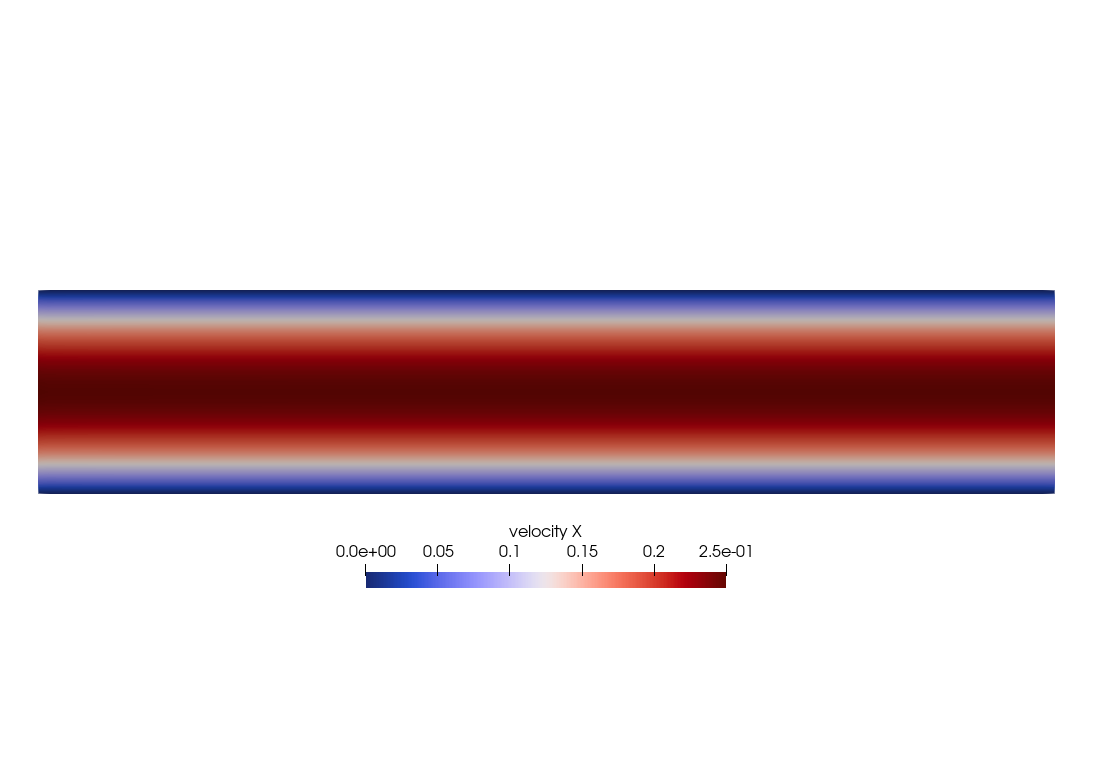
\includegraphics[width=4.5cm]{images/mms/jolm17/u}
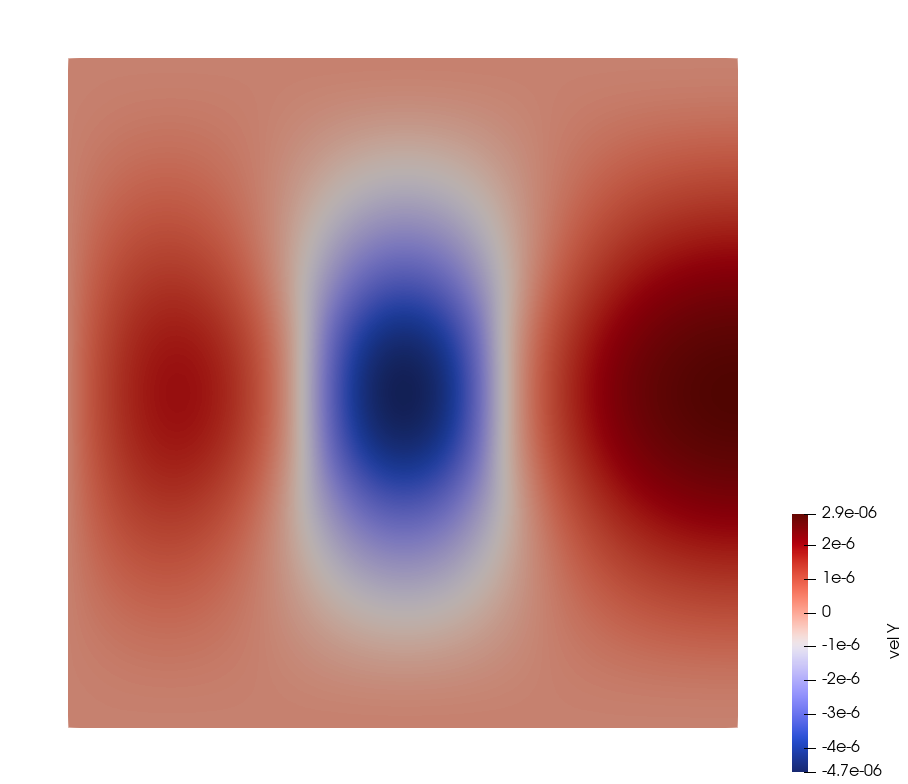
\includegraphics[width=4.5cm]{images/mms/jolm17/v}
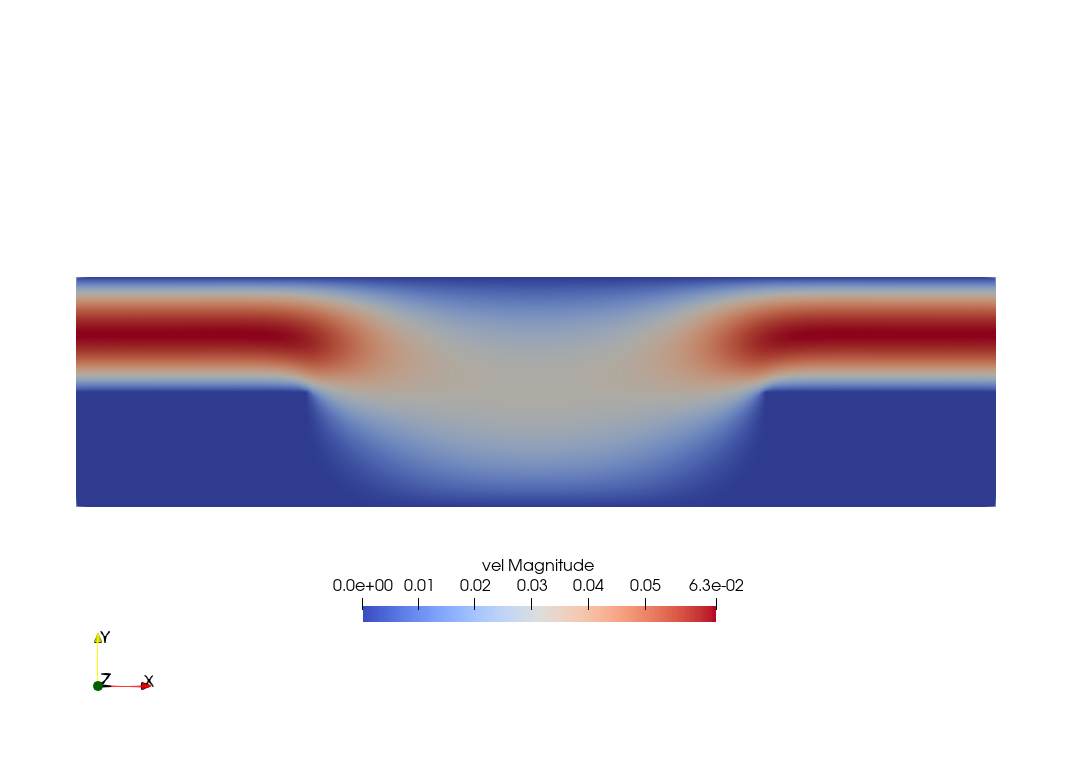
\includegraphics[width=4.5cm]{images/mms/jolm17/vel}\\
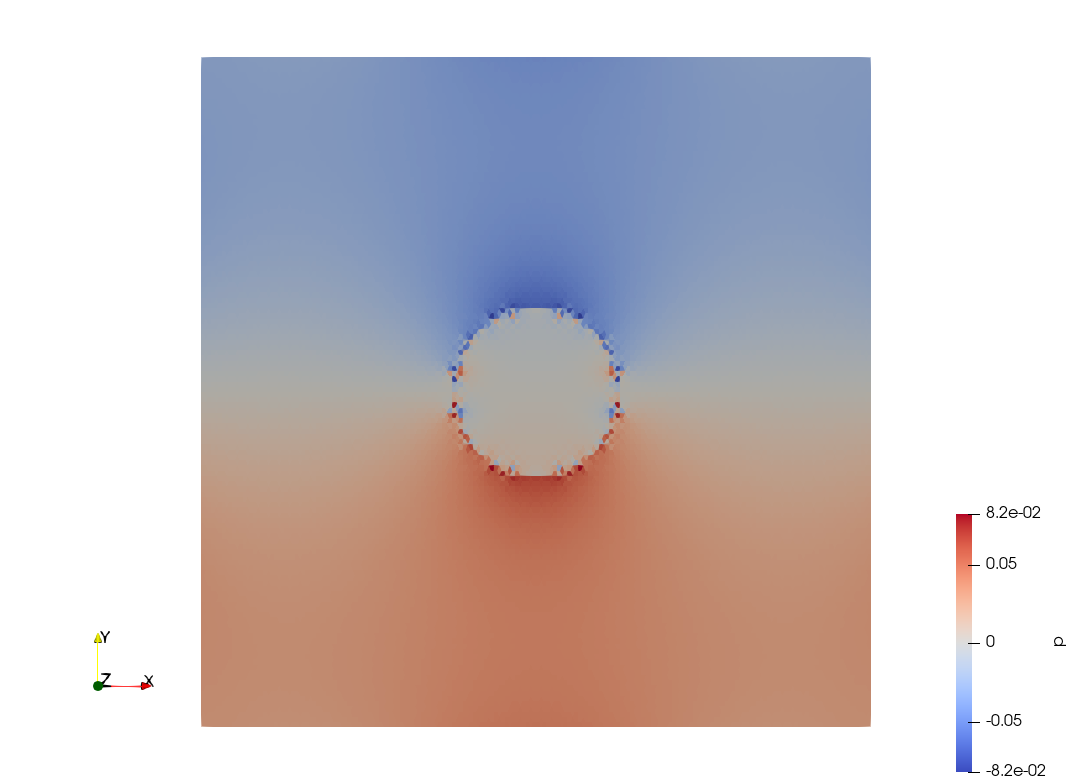
\includegraphics[width=4.5cm]{images/mms/jolm17/p}
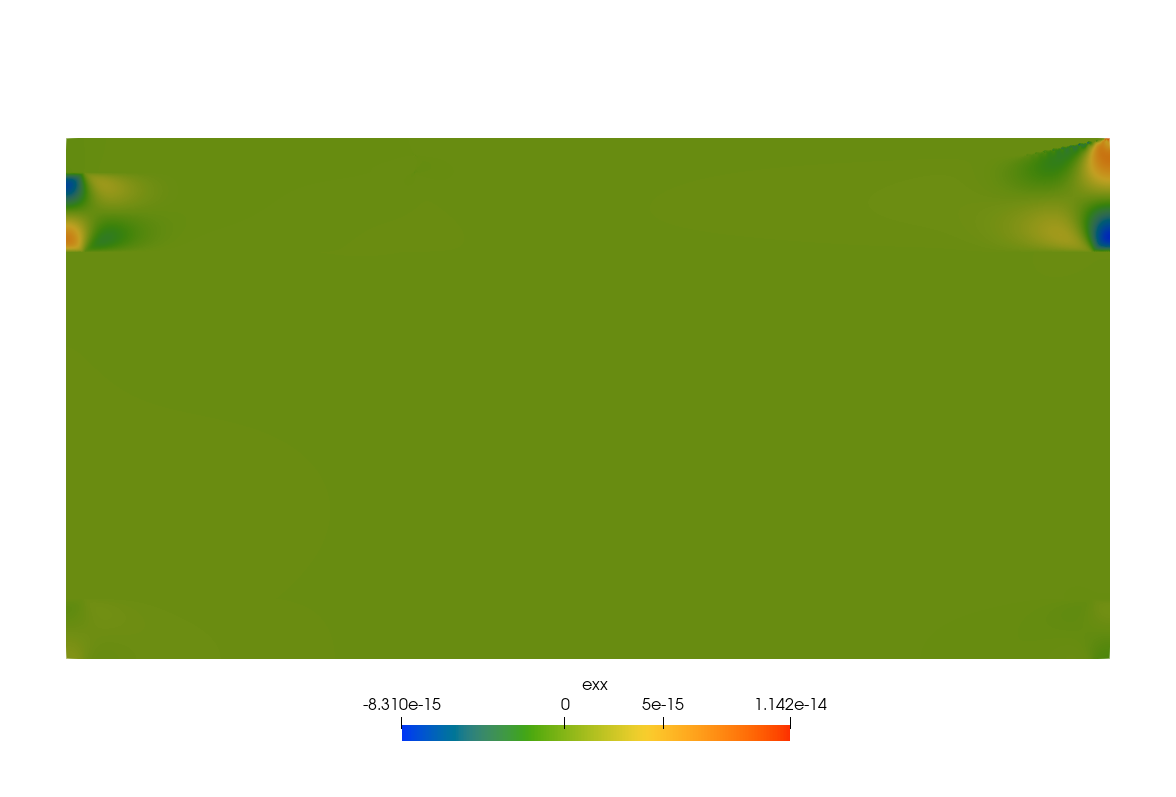
\includegraphics[width=4.5cm]{images/mms/jolm17/exx}
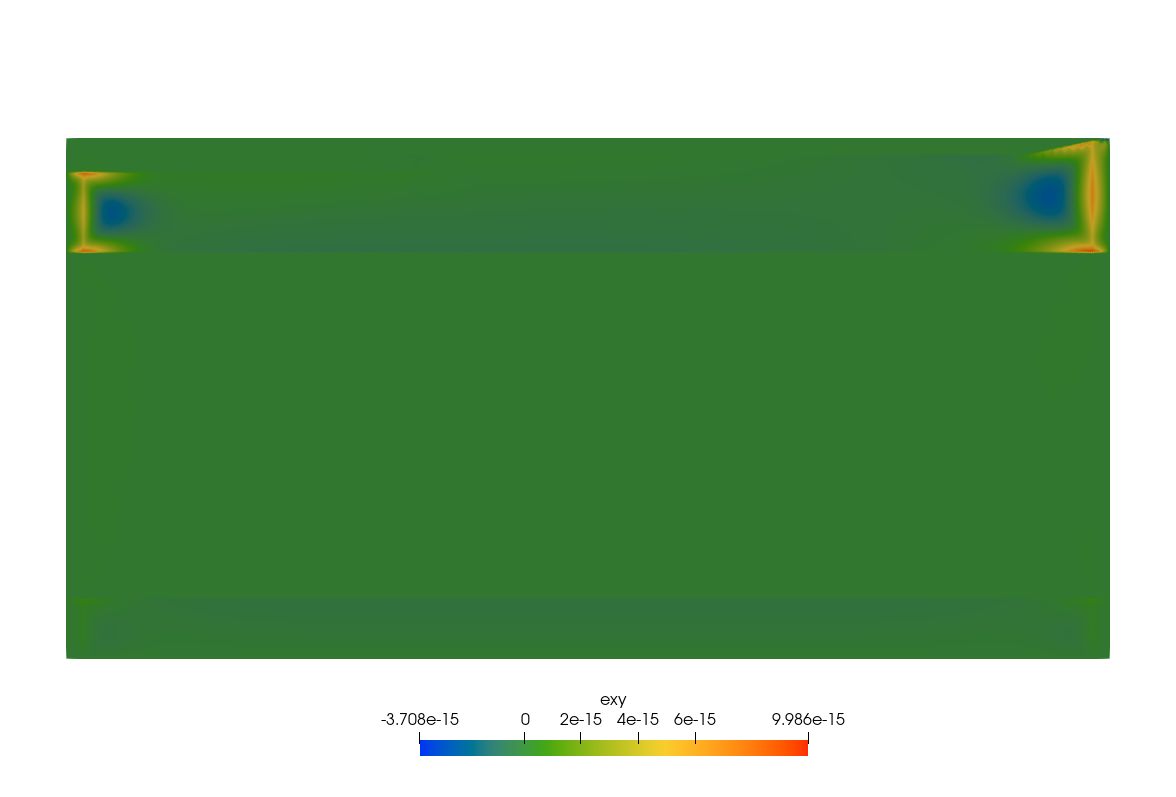
\includegraphics[width=4.5cm]{images/mms/jolm17/exy}
\end{center}

---------------------------------------------------------

At some point I had also written this about he very same benchmark.
The velocity is given by
\begin{eqnarray}
\upnu_x &=&200 x^2(1-x)^2 y (1-y)(1-2y) = 100 a(x) a'(y) \nn\\
\upnu_y &=& - 200 x(1-x)(1-2x)y^2(1-y)^2 = -100 a'(x) a(y) \nn
\end{eqnarray}
with 
\begin{eqnarray}
a(x)  &=& x^2(1-x)^2 \nn\\
a'(x) &=& 2x(1-x)^2-2x^2(1-x) = 2x(1-x)(1-2x) \nn\\
a''(x) &=& 2(1-6x+6x^2) \nn\\
a'''(x) &=& 24x-12 \nn
\end{eqnarray}
We can now compute the components of the strain rate tensor:
\begin{eqnarray}
\dot{\varepsilon}_{xx}=
\frac{\partial \upnu_x}{\partial x}
&=&\frac{\partial  (100 a(x)a'(y))}{\partial x} =
100 a'(x)a'(y) \nonumber\\
\dot{\varepsilon}_{yy}=
\frac{\partial \upnu_y}{\partial y}
&=& \frac{\partial (-100 a'(x) a(y))}{\partial y}
= -100 a'(x)a'(y) \nonumber\\
\dot{\varepsilon}_{xy}=
\dot{\varepsilon}_{yx}=
\frac12 \left( \frac{\partial \upnu_x}{\partial y}
+\frac{\partial \upnu_y}{\partial x} \right) &=& 
\frac12 \left(100 a(x)a''(y) -100 a''(x) a(y) \right) 
= 50 \left( a(x)a''(y) - a''(x) a(y) \right)
\nonumber
\end{eqnarray}
The momentum conservation equation is given by
\begin{eqnarray}
- \partial_x p + \partial_x (2\eta \dot{\varepsilon}_{xx})
+ \partial_y (2\eta \dot{\varepsilon}_{xy}) + b_x &=&0 \nn\\
- \partial_y p + \partial_x (2\eta \dot{\varepsilon}_{xy})
+ \partial_y (2\eta \dot{\varepsilon}_{yy}) + b_y &=&0 \nn
\end{eqnarray}
Then 
\begin{eqnarray}
b_x 
&=& \partial_x p - \partial_x (2\eta \dot{\varepsilon}_{xx}) 
- \partial_y (2\eta \dot{\varepsilon}_{xy}) \nn\\
&=& \partial_x p - \partial_x [2 \eta 100 a'(x)a'(y) ]
- \partial_y [2 \eta 50 \left( a(x)a''(y) - a''(x) a(y) \right) ] \nn\\
&=& \partial_x p -  200 \eta a''(x)a'(y) - 
100\eta [ a(x)a'''(y) - a''(x)a'(y)] \nn\\
&=& \partial_x p - 100 \eta a''(x)a'(y) - 100\eta  a(x)a'''(y) \nn\\ 
&=& \partial_x p - 100 \eta [a''(x)a'(y) + a(x)a'''(y) ]
\nonumber\\ \nonumber\\
b_y 
&=&  \partial_y p - \partial_x (2\eta \dot{\varepsilon}_{xy}) 
- \partial_y (2\eta \dot{\varepsilon}_{yy}) \nn\\
&=&  \partial_y p - \partial_x 
[2\eta  50 \left( a(x)a''(y) - a''(x) a(y) \right) ]
+ \partial_y 2 \eta 100 a'(x)a'(y) \nn\\
&=&  \partial_y p - 100\eta (a'(x)a''(y) -a'''(x) a(y)  ) + 200 \eta a'(x)a''(y)\nn \\ 
&=&  \partial_y p + 100 \eta a'(x)a''(y) + 100 \eta a'''(x) a(y) \nonumber\\
&=& \partial_y p + 100 \eta [ a'(x)a''(y) +  a'''(x) a(y) ] \nonumber
\end{eqnarray}
with 
\begin{eqnarray}
p(x,y)&=&10
\left[
\left(x-\frac12\right)^3y^2
+(1-x)^3\left(y-\frac12\right)^3  
\right]
\nonumber\\
\frac{\partial p}{\partial x} &=& 10 \left[3 \left(x-\frac12\right)^2 y^2
-3 (1-x)^2 \left(y-\frac12\right)^3  \right] \nonumber\\
\frac{\partial p}{\partial y}  &=& 10 \left[  
\left(x-\frac12\right)^3 2y
+(1-x)^33 \left(y-\frac12\right)^2
\right] \nonumber
\end{eqnarray}

See \stone~104.







